\documentclass{article}

% NeurIPS 2026 template from the course formatting ZIP.
% preprint shows author names; the style file itself is unchanged.
\PassOptionsToPackage{numbers,sort&compress}{natbib}
\usepackage[preprint]{neurips_2026}

\usepackage[utf8]{inputenc}
\usepackage[T1]{fontenc}
\usepackage{hyperref}
\usepackage{url}
\usepackage{booktabs}
\usepackage{amsfonts}
\usepackage{nicefrac}
\usepackage{microtype}
\usepackage{xcolor}
\usepackage{graphicx}
\usepackage{array}
\usepackage{float}
\setlength{\tabcolsep}{4pt}

\hypersetup{hidelinks,pdftitle={LearnLoop Project Proposal},pdfauthor={Group 72}}

% Coursework notice only. neurips_2026.sty is the file supplied in the template ZIP.
\makeatletter
\renewcommand{\@noticestring}{COMP7608B Project Proposal}
\makeatother

\title{[Group 72] LearnLoop\\A Stateful Agentic Platform for Adaptive Learning}

\author{Fong Chi Ching, Ching Nok Yee, Lai Hok Lam Justin, Zhou Yuxin}

\begin{document}

\maketitle

% The course proposal guideline requires no abstract.



\section{Group Members}

\begin{tabular}{@{}lll@{}}

\toprule

\textbf{Name} & \textbf{Student ID} & \textbf{Email} \\

\midrule

Fong Chi Ching & 3035299466 & u3529946@connect.hku.hk \\

Ching Nok Yee & 3035283572 & u3528357@connect.hku.hk \\

Lai Hok Lam Justin & 3036657081 & u3665708@connect.hku.hk \\

Zhou Yuxin & 3036791693 & u3679169@connect.hku.hk \\

\bottomrule

\end{tabular}

\section{Project Objective}

This project aims to build LearnLoop, an agentic learning platform that turns a student's uploaded course materials into an adaptive, persistent learning journey. Given a set of documents and a learner-defined goal, LearnLoop decides what the learner should do next and whether they have understood it, revising the plan as evidence accumulates across learning sessions. The deliverable of this project is a working end-to-end system comprising three Artificial Intelligence (AI) agents, neither a model nor a single prompt (Section 4).

We pursue three objectives:
\begingroup
\setlength{\topsep}{2pt}
\setlength{\itemsep}{1pt}
\setlength{\parsep}{0pt}
\begin{enumerate}

\item Decide the next best action. A source-grounded agent--environment loop, informed by ReAct \citep{ref1}, proposes an educational action, the runtime validates and executes it, and the observation informs the next decision.

\item Ground decisions in course content. LearnLoop derives learning items and prerequisites from the uploaded materials and maintains concept-level learner evidence and reusable learning activities within the selected course unit.

\item Verify and track progress. Actions and assessment evidence are validated before persistence. Advancement to demonstrated status requires repeated rubric-meeting evidence; other validated outcomes may update diagnostic states. Durable checkpoints allow interrupted sessions to resume.

\end{enumerate}
\endgroup

For evaluation, we will develop controlled LLM-based pseudo-students to compare agent prompt variants. The selected LearnLoop configuration will also be compared with a fixed-sequence tutor and a tutor without cross-session learner memory, measuring learning quality, learner-state accuracy, trajectory quality, workflow robustness, latency and cost (Section 5 and Appendix C2).

\section{Motivation and Challenges}

Students often receive course outlines, slides, and readings but are unsure where to start, which ideas matter most, or what they need to understand first. They may review familiar topics while overlooking gaps in their knowledge. Asking a chatbot to explain a topic is possible, but the quality depends heavily on how the question is phrased. It is also hard to keep track of their own progress.

LearnLoop addresses this by organizing uploaded materials into a learning path, checking what students understand, and offering practice or explanations where needed. By remembering earlier attempts, it revisits difficult topics and adjusts the plan over time. Research on intelligent tutoring systems supports this approach \citep{ref2}. We will evaluate whether LearnLoop selects useful activities and helps students navigate their materials more confidently.

The main challenges are (i) recognizing a lasting misunderstanding rather than a temporary mistake, (ii) finding reliable support in the uploaded materials, and (iii) keeping an accurate record of progress. We will validate assessment evidence before updating the learner's state, allow the system to express uncertainty, and limit repeated attempts when tools fail. Missions and rewards will support the learning tasks, while progress will depend on demonstrated understanding. Research on gamification motivates these supporting features \citep{ref3}; motivation and engagement effects remain outside the controlled simulator evaluation.

\section{Potential Solutions}

\subsection{Knowledge Graph Based Multi Agent Architecture}

LearnLoop will use three specialized agents within a shared agentic workflow: an Expert Agent, a Tutoring Agent, and an Assessing Agent. Together, they will follow a continuous construct, teach, assess, and adapt cycle. Each agent will have distinct responsibilities and tools, while a shared runtime will manage state, validate outputs, and record execution traces. Appendix A shows the architecture and validated feedback loop.

The Expert Agent will process uploaded course materials and construct a source-grounded knowledge graph. Each node will represent a course concept, while edges will represent prerequisite, dependency, or related-topic relationships. The agent will also generate explanations, examples, questions, hints, reference answers, and assessment rubrics at three difficulty levels: basic (recall and direct conceptual understanding), intermediate (application, comparison, and explanation), and advanced (analysis and multi-concept reasoning). Supporting course passages will be retrieved using retrieval-augmented generation \citep{ref4}.

Optional external enrichment is a future extension, excluded from prototype teaching, assessment and experiments. It would use a separate retrieval interface and retain external-source references. The optional enrichment label in Appendix A denotes this extension; Appendix B specifies the course-grounded prototype tools.

The Tutoring Agent will select the next concept, activity, and difficulty according to the course knowledge graph and the learner's current state. Candidate concepts will first be filtered according to prerequisite readiness and then ranked using learner need, assessment uncertainty, review urgency, and recent performance. The agent may introduce an unassessed concept, provide further practice, adjust question difficulty, revisit a prerequisite, reassess a review-due concept, or advance the learner to a related concept.

The Assessing Agent will evaluate learner responses using rubric coverage, question difficulty, response time, hint usage, previous attempts, and contradictory evidence. Correctness and rubric coverage will provide the primary evidence, while the remaining signals will adjust the strength of that evidence. The agent will record misconceptions and propose learner-state updates, but a deterministic runtime will validate each update before committing it.

\subsection{Difficulty Aware Learner Model}

LearnLoop will be designed to map learner's knowledge on a knowledge graph generated by course materials. Upon publishing, the concept-connected knowledge graph will be shared across learners, while each learner will have separate concept-level assessment evidence and progress states. This persistent evidence model is inspired by knowledge tracing \citep{ref5}. The prototype will use explicit transition rules.

Each concept will retain one overall state: unassessed (insufficient evidence), developing (partial understanding or supported success), demonstrated (sufficient independent evidence at the required difficulty), or review\_due (previously demonstrated understanding needs reassessment).

Because performance may differ by question difficulty, evidence is stored separately for basic, intermediate, and advanced activities, including independent and hint-assisted attempts, response times, misconceptions, contradictions, and the last assessment and review dates. A learner may be demonstrated at the basic level, developing at the intermediate level, and unassessed at the advanced level. The overall concept state is relative to that concept's target difficulty.

Demonstrated status requires two rubric-meeting responses to distinct questions at the target difficulty, without hints or unresolved contradictions. Validated incorrect, partial or hinted performance supports developing status. Later errors preserve evidence: inconclusive contradictions move demonstrated concepts to review\_due; confirmed weakness moves them to developing. Demonstrated concepts become review\_due after seven days, using simulated time in experiments. Prerequisite readiness requires demonstrated status at the prerequisite's target difficulty. These rules will be fixed before evaluation.

\subsection{Autonomous Learning Loop and Runtime Control}

After the Expert Agent prepares the knowledge graph and resources, the Tutoring Agent will select a concept, activity, and difficulty from the graph and learner state. Following ReAct \citep{ref1}, tool outcomes and assessment observations will inform each subsequent decision.

After an activity, the Assessing Agent will propose a concept-state update using the evidence described above. The runtime will validate source support, prerequisite relationships, and the permitted transition before committing it. The updated state will become a new observation for the Tutoring Agent. Retained assessment feedback and diagnostic summaries will support adaptation across sessions. This draws inspiration from Reflexion's use of feedback and episodic reflection \citep{ref6}, while LearnLoop uses explicit learner evidence and deterministic state-transition rules.

The loop will respond to rapid progress, persistent misconceptions, hint dependence, difficulty-specific weaknesses, conflicting evidence, and knowledge decay. It may adjust difficulty, provide targeted remediation, revisit prerequisites, schedule review, or advance. Typed tool contracts, version checks, unique operation IDs, and durable checkpoints will support validated execution and session resumption. Bounded retries and explicit insufficient-evidence outcomes will control failures; the runtime will pause for learner input or stop at execution limits.

Structured traces will record decisions, tool calls, evidence, proposed and committed updates, latency, token consumption, and cost. AgentBench motivates evaluating agents through multi-step interactions \citep{ref7}; LearnLoop will use its own course-specific scenarios and trajectory rubric rather than claim to run the AgentBench benchmark. Appendix B provides tool contracts; Appendix C provides acceptance cases.

\subsection{Technology and Implementation}

The frontend will use Next.js, TypeScript, and React components \citep{ref8} to show activities, source references, and progress. A Python FastAPI backend will run the three agents in one LangGraph workflow, with conditional handoffs and checkpoints for assessment, remediation, review, and interrupted sessions \citep{ref9}. OpenRouter will provide the language model, with the model identifier and generation settings fixed for each experiment. Overlapping passages will be embedded with BAAI/bge-m3, initially selected for multilingual retrieval and 1,024-dimensional vectors \citep{ref10}, and indexed in Qdrant with document IDs, source locations, and course-access metadata \citep{ref11}. PostgreSQL will store the concept graph, learner evidence, plans, and checkpoints; Qdrant will remain the retrieval index. Schema validation will enforce tool contracts and state transitions, and Docker Compose will support reproducible deployment.

\section{Experimental Dataset Description and Evaluation Plan}

\subsection{Course Dataset and Learning Resources}

The initial dataset will consist of selected COMP7608B course materials, limited to one coherent course unit of approximately 10 to 20 concepts and their relationships. The Expert Agent will generate the source-grounded graph and the teaching resources in Section 4.1, and nodes, edges, questions, and rubrics will retain links to the supporting course passages. Model-based screening using multi-model agreement, embedding similarity, and LLM-as-judge scoring will flag items for inspection. The group will manually review every flagged item and a sample of unflagged items for conceptual correctness, source grounding, prerequisite accuracy, and appropriate difficulty. Test questions used for final evaluation will be excluded from the agents' retrieval and teaching resources.

\subsection{Prompt Configurations for Evaluation}

For evaluation, three prompt variants will be generated per agent to form a 3$\times$3$\times$3 factorial design with 27 configurations. Expert prompts will vary structural guidance, grounding, and verification; Tutoring prompts will use state-based, graph-aware, or utility-based selection; and Assessing prompts will use correctness-focused, evidence-weighted, or conservative assessment. Model versions, tools, schemas, course information, and activity budgets will remain fixed to isolate prompting effects.

\subsection{Controlled Learner Simulation}

Each configuration will interact with the same controlled LLM-based pseudo-students. Hidden profiles will specify initial knowledge, difficulty-specific ability, misconceptions, hint dependence, response characteristics, and memory of prior teaching. Profiles will cover novice, intermediate, misconception-prone, and hint-dependent learners. Simulator states will remain separate from LearnLoop's estimates, enabling learner-state accuracy checks. Before each learning episode, the pseudo-student completes a pre-test covering the same concepts as the post-test; the pre-test results initialise LearnLoop's estimate of the learner's knowledge state. Each configuration will be run repeatedly with the same initial states, activity limits, and stopping conditions to reduce stochastic variation.

\subsection{Evaluation Measures}

We will evaluate four dimensions using the measures below.

{\small
\begin{tabular}{@{}>{\raggedright\arraybackslash}p{0.22\linewidth}>{\raggedright\arraybackslash}p{0.74\linewidth}@{}}
\toprule
\textbf{Measure} & \textbf{Definition or assessment} \\
\midrule
Learning quality & Performance on an unseen post-test, concepts mastered, learning gain per activity, and activities required to reach the target performance \\
Learner-state accuracy & Agreement between LearnLoop's estimated states and the pseudo-student's hidden states, including macro F1, difficulty estimation, misconception detection, and false-demonstration rate \\
Trajectory quality & Appropriateness of concept selection, prerequisite consistency, difficulty suitability, evidence use, state-update validity, redundancy, and recovery from uncertainty \\
Operational performance & Input and output tokens, monetary cost, cost per mastered concept, end-to-end latency, and median and p95 latency by agent \\
\bottomrule
\end{tabular}
}

A fixed, unseen post-test with questions at multiple difficulty levels will be scored independently of the experimental Assessing Agent, so a lenient assessor cannot establish demonstrated status on its own. Traces will record available evidence, candidate and selected actions, tool calls, concept and difficulty choices, proposed and committed state changes, errors, retries, tokens, latency, and cost. A common rubric and deterministic checks will flag prerequisite violations, invalid transitions, repeated actions, and unsupported mastery updates.

\subsection{Controls and Analysis}

Configurations will share learner profiles, model settings, turn limits, post-test criteria, tool permissions, and runtime budgets. The graph, resources, and activity pool stay fixed within each Expert variant and may differ across variants built from the same materials. Analysis will estimate prompt effects and interactions on quality, learner-state accuracy, trajectory quality, latency, and cost, and will identify the quality-efficiency frontier. If full evaluation is too expensive, all 27 configurations will receive a short screen, and only the strongest non-dominated configurations will be evaluated repeatedly in full.

\label{main-end}

\clearpage

\appendix

\section{System Architecture}

\subsection{Overall Architecture}

The architecture below shows the course preparation stage and the adaptive learning loop. The Expert Agent supplies a shared course knowledge base. The Tutoring Agent uses course evidence and current learner state to select an activity. The Assessing Agent evaluates the learner's response against the rubric and course sources. Only a validated runtime commit changes the persistent learner model, which informs the next tutoring decision.

\begin{figure}[H]
\centering
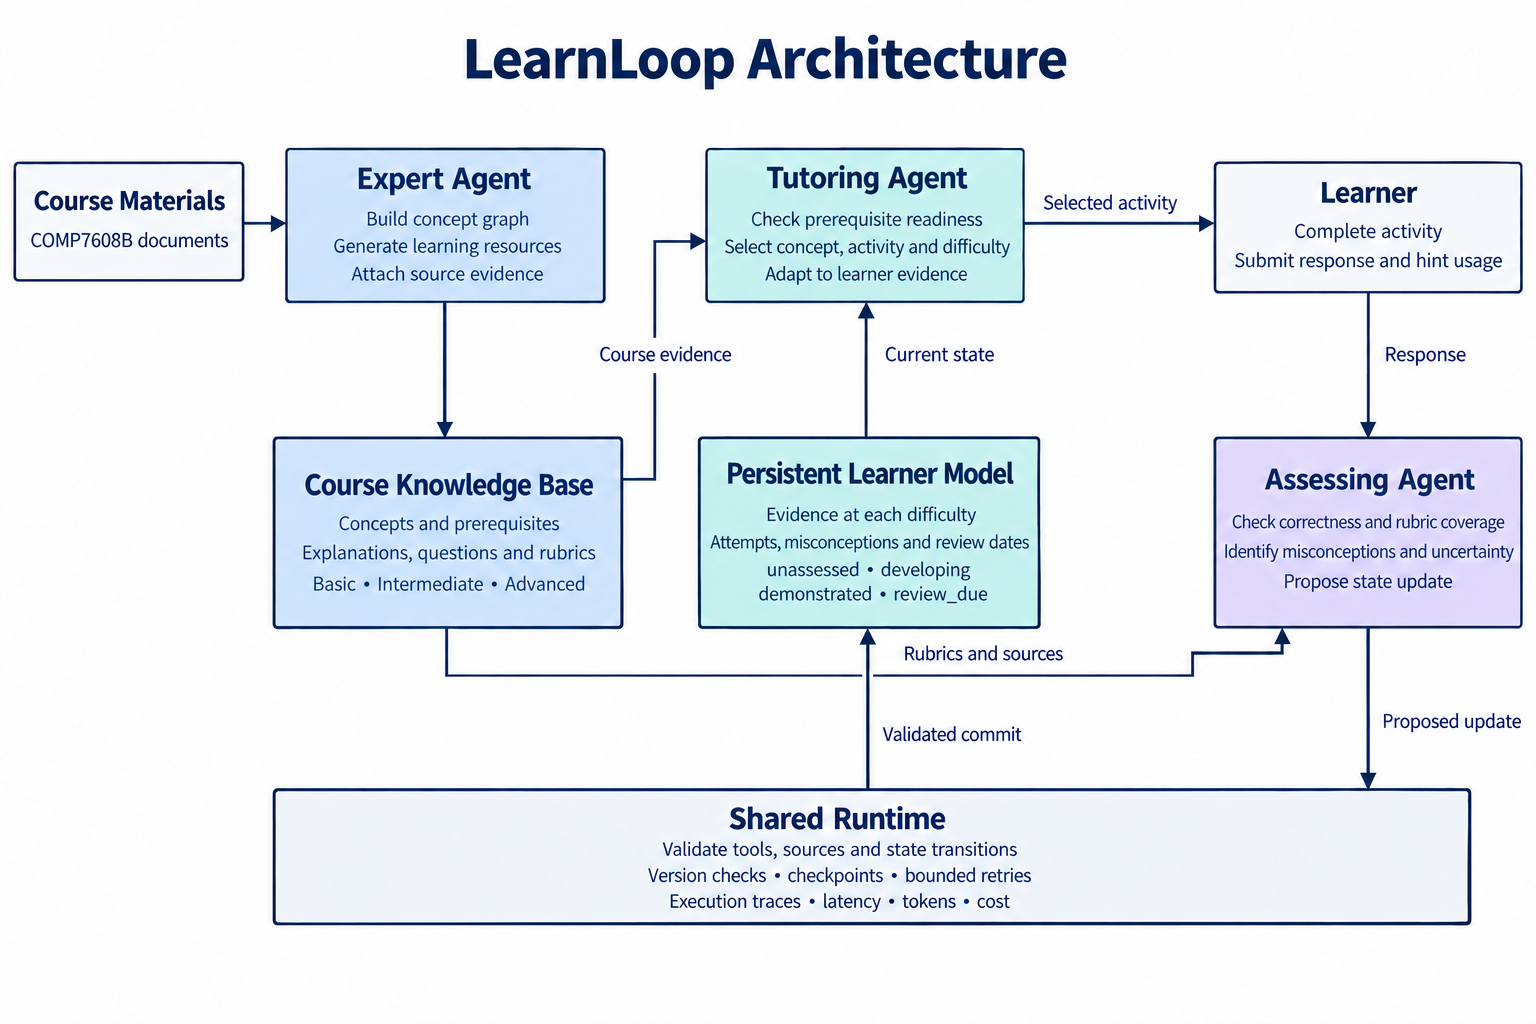
\includegraphics[width=\linewidth]{figures/overall}
\caption{Overall architecture of LearnLoop.}
\end{figure}

The shared runtime also validates tool actions, checks record versions, maintains checkpoints, bounds retries, and logs latency, token use and cost. Missions and rewards remain supporting interface features; they do not form a fourth agent or determine learner-state transitions.

\clearpage
\subsection{Expert Agent}

The Expert Agent prepares one course unit before tutoring begins. It retrieves course-scoped passages, proposes concepts with prerequisite and related-topic edges, and generates explanations, questions, hints, reference answers and rubrics at basic, intermediate and advanced difficulty. Nodes, edges and resources keep links to the supporting passages. The runtime checks source references, prerequisite cycles, and difficulty and rubric fields, then publishes a versioned course knowledge base. If the retry limit is reached or no supporting evidence remains, the run stops and the item is flagged for review. Optional external enrichment stays separate from this course-grounded path.

\begin{figure}[H]
\centering
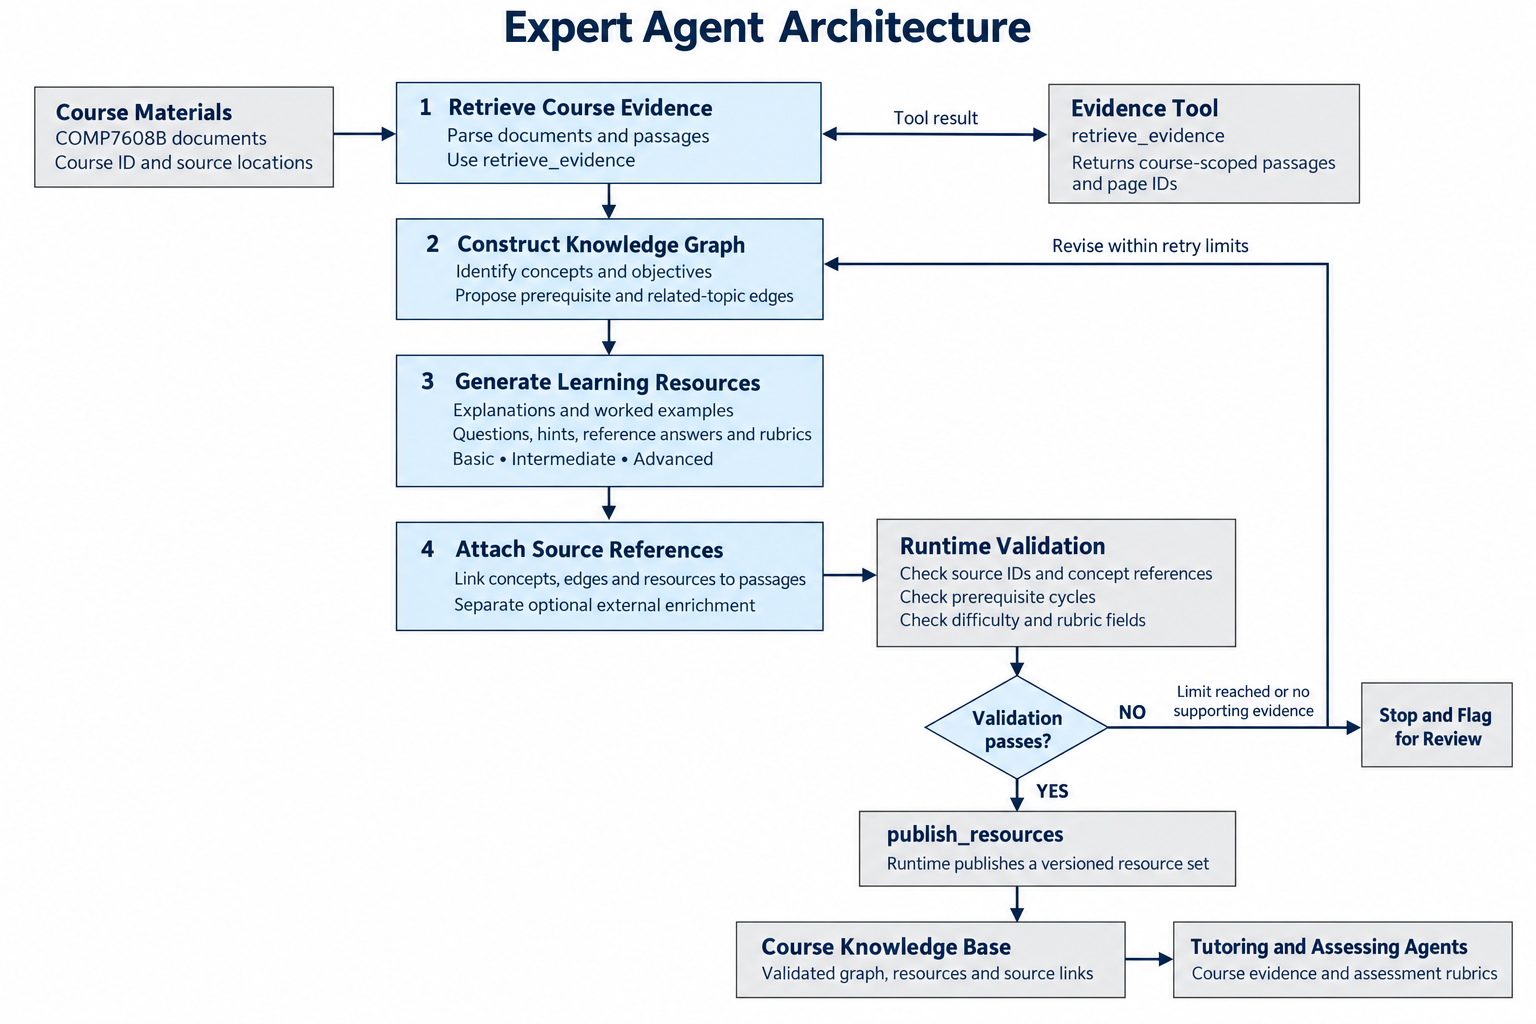
\includegraphics[width=\linewidth]{figures/expert}
\caption{Expert Agent workflow.}
\end{figure}

\clearpage
\subsection{Tutoring Agent}

The Tutoring Agent selects the next activity from the published course knowledge base and the persistent learner model. It loads the learner state and relevant passages, removes concepts whose prerequisites are not demonstrated at the target difficulty, and ranks the rest by learner need, assessment uncertainty, review urgency and recent performance. The selected action may introduce a concept, assign practice, change difficulty, revisit a prerequisite, schedule review or advance. The runtime checks the objective, sources, prerequisites, ownership and record version before it persists the activity and plan. An invalid proposal is replanned within the retry budget. Missing evidence or an exhausted budget pauses the session and keeps the current progress. The learner state updated by assessment is the next observation.

\begin{figure}[H]
\centering
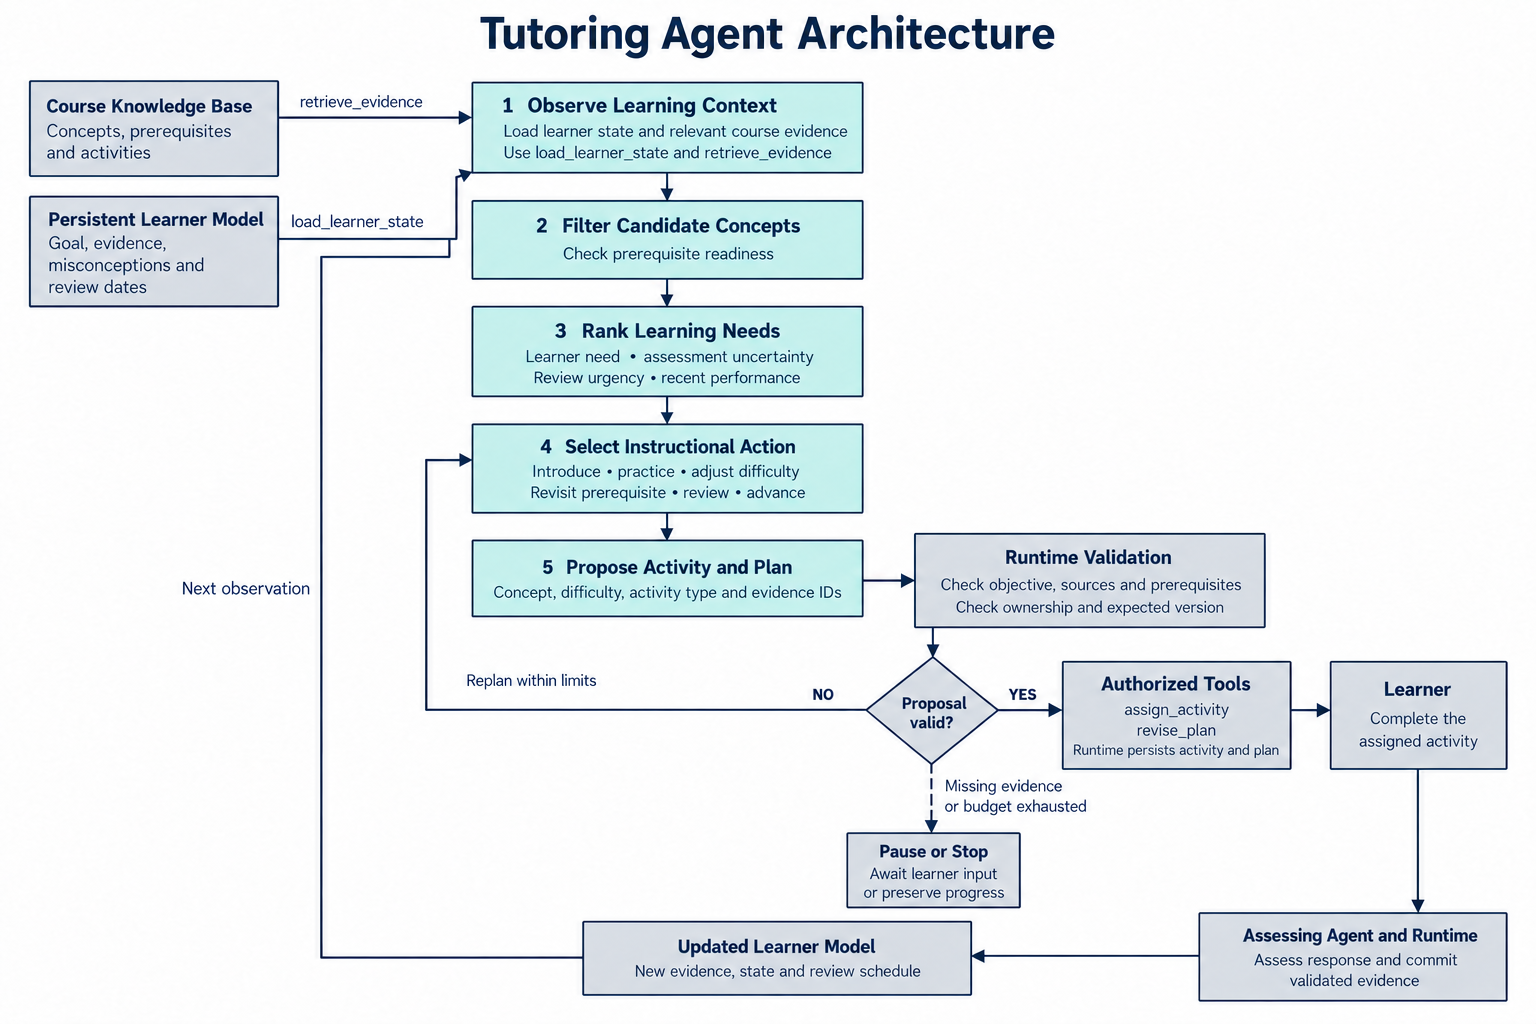
\includegraphics[width=\linewidth]{figures/tutoring}
\caption{Tutoring Agent workflow.}
\end{figure}

\clearpage
\subsection{Assessing Agent}

The Assessing Agent grades the learner response against the activity rubric and course sources. Correctness and rubric coverage are the primary evidence. Difficulty, hint use, response time, prior attempts and contradictions only qualify that evidence. When the evidence is sufficient, the agent proposes a state update at the concept's target difficulty and retains every assessment record. The runtime commits the update only if the rubric, sources, record version and Section 4.2 rules hold, including two independent target-difficulty responses before demonstrated status. Insufficient evidence or an unsupported or stale update is stored as uncertainty and does not advance the concept. If no further evidence can be gathered, the session pauses with progress saved. A committed state is the next observation for the Tutoring Agent.

\begin{figure}[H]
\centering
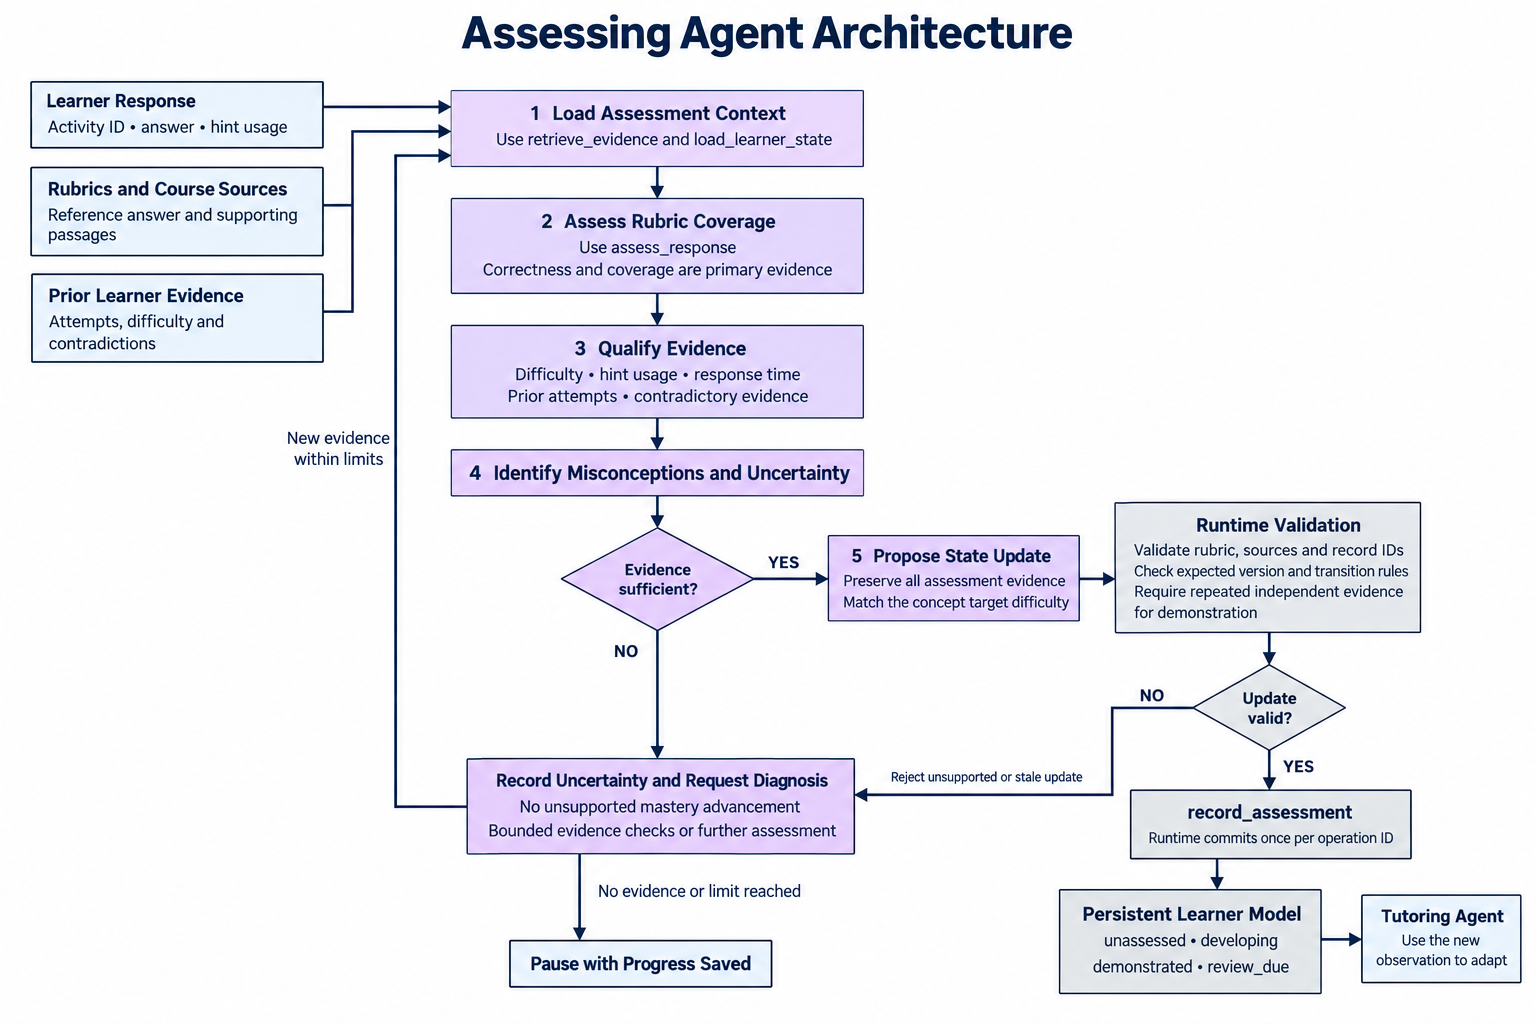
\includegraphics[width=\linewidth]{figures/assessing}
\caption{Assessing Agent workflow.}
\end{figure}

\clearpage

\section{Agent Responsibilities and Runtime Contracts}

These planned interfaces define how the three agents use the shared course knowledge base and persistent learner model. Agents propose actions and evidence; the runtime authorizes tools and commits validated writes. All records are scoped to the authorized course and learner.

\subsection{Agent Responsibilities}

{\small
\begin{tabular}{@{}>{\raggedright\arraybackslash}p{0.14\linewidth}>{\raggedright\arraybackslash}p{0.42\linewidth}>{\raggedright\arraybackslash}p{0.40\linewidth}@{}}
\toprule
\textbf{Agent} & \textbf{Inputs and responsibilities} & \textbf{Output and handoff} \\
\midrule
Expert & Course documents and source passages; extract concepts and prerequisites, then generate resources at three difficulty levels. & Proposed graph and resources with passage references; runtime validates before publication. \\
\addlinespace[2pt]
Tutoring & Validated graph, learner evidence, goal and review schedule; filter by prerequisites and select concept, activity and difficulty. & Activity proposal with objective, evidence and rationale; runtime assigns the activity to the learner. \\
\addlinespace[2pt]
Assessing & Learner response, activity rubric, source passages, hint usage and previous evidence; assess coverage and uncertainty. & Assessment evidence, misconceptions and candidate state update; runtime validates and commits. \\
\bottomrule
\end{tabular}
}

\subsection{Shared Tool Contracts}

Every tool returns a status, evidence or result identifiers, and a structured error when unsuccessful. Write operations use an operation\_id and, where applicable, an expected\_version; retries return the original committed result rather than duplicating it.

{\small
\begin{tabular}{@{}>{\raggedright\arraybackslash}p{0.24\linewidth}>{\raggedright\arraybackslash}p{0.34\linewidth}>{\raggedright\arraybackslash}p{0.38\linewidth}@{}}
\toprule
\textbf{Tool and caller} & \textbf{Input contract} & \textbf{Result and runtime checks} \\
\midrule
retrieve\_evidence\newline All agents & course\_id, query, optional concept\_id or document\_ids & Source passages and page IDs; enforce course scope and retrieval limits. Course preparation may retrieve before concept IDs exist. Empty results preserve an evidence gap. \\
\addlinespace[2pt]
publish\_resources\newline Expert & operation\_id, course\_id, graph, resources, source\_ids & Versioned graph and resource IDs; check source references, concept IDs, prerequisite cycles, and rubric/difficulty fields. \\
\addlinespace[2pt]
load\_learner\_state\newline Tutoring or Assessing & learner\_id, concept\_ids & Selected evidence records, learner goal, review dates and version; enforce learner ownership and course scope before loading context. \\
\addlinespace[2pt]
assign\_activity\newline Tutoring & operation\_id, learner\_id, concept\_id, resource\_id, difficulty, activity\_type, evidence\_ids, expected\_version & Persisted activity ID; validate prerequisite readiness, objective, resource, difficulty and learner-state version. Duplicate operation IDs reuse the prior result. \\
\addlinespace[2pt]
assess\_response\newline Assessing & activity\_id, response, hint\_used, response\_time\_ms, prior\_evidence\_ids & assessment\_id, rubric coverage, correctness, misconceptions and uncertainty; validate activity, rubric and source references. Runtime records elapsed response time; persisted assessment results supply the ID used by record\_assessment. \\
\addlinespace[2pt]
record\_assessment\newline Assessing via runtime & operation\_id, learner\_id, expected\_version, assessment\_id, candidate\_update & Committed evidence and permitted concept state; reject stale versions and unsupported demonstration. \\
\addlinespace[2pt]
revise\_plan\newline Tutoring & operation\_id, learner\_id, expected\_version, activity\_ids, review\_dates & New plan version; check ownership, prerequisites and referenced activities before transactional write. \\
\bottomrule
\end{tabular}
}

\subsection{Learner State and Persistence}

Each concept record will retain the target difficulty, overall state, evidence at basic/intermediate/advanced levels, independent and hinted attempts, rubric results, misconceptions, contradictions, timestamps and review dates. Assessment evidence, including uncertain outcomes, will be appended rather than overwritten. The runtime will derive overall status against the target difficulty using the fixed rules in Section 4.2. Uncertainty may be persisted without advancing the concept state.

{\small
\begin{tabular}{@{}>{\raggedright\arraybackslash}p{0.18\linewidth}>{\raggedright\arraybackslash}p{0.78\linewidth}@{}}
\toprule
\textbf{State} & \textbf{Entry or transition rule} \\
\midrule
unassessed & No validated diagnostic assessment evidence is available at the target difficulty. \\
\addlinespace[2pt]
developing & Incorrect, partial or hint-assisted performance indicates a gap; further independent evidence is needed. Confirmed weakness may move a demonstrated concept here. \\
\addlinespace[2pt]
demonstrated & At least two independent responses to distinct questions meet the rubric at the target difficulty, without hints or unresolved contradictions. \\
\addlinespace[2pt]
review\_due & A demonstrated concept reaches its seven-day review date or an inconclusive contradiction requires reassessment; earlier evidence remains available. \\
\bottomrule
\end{tabular}
}

Pending activities, committed evidence, plan versions and operation results will be saved at durable checkpoints. Timeouts, restarts and retry exhaustion will leave a resumable status. Response time and hint usage may qualify evidence strength but will not independently establish demonstrated understanding.

\clearpage

\section{Verification and Evaluation Details}

\subsection{Planned Acceptance Cases}

These cases check the transition rules in Section 4.2 and the deterministic checks in Section 5.4. They are planned tests of proposed versus committed actions, not reported results.

{\small
\begin{tabular}{@{}>{\raggedright\arraybackslash}p{0.28\linewidth}>{\raggedright\arraybackslash}p{0.68\linewidth}@{}}
\toprule
\textbf{Case} & \textbf{Expected behavior} \\
\midrule
Unsupported course resource & A concept, relationship or rubric without valid source evidence is rejected or flagged for review before use. \\
\addlinespace[2pt]
Prerequisite violation & An activity is blocked unless the prerequisite is demonstrated at its target difficulty. The Tutoring Agent receives the reason and selects remediation. \\
\addlinespace[2pt]
Hint or partial success & A hinted or partial answer is stored as developing evidence and cannot by itself support demonstrated status. \\
\addlinespace[2pt]
Single success or pre-test only & One rubric-meeting response, including the pre-test that initialises the estimate, does not set demonstrated status. Demonstrated status requires two independent responses to distinct questions at the target difficulty, without hints or unresolved contradictions. \\
\addlinespace[2pt]
Difficulty mismatch & Success below the concept's target difficulty does not demonstrate that target. Evidence stays separated by basic, intermediate and advanced difficulty. \\
\addlinespace[2pt]
Contradictory evidence & A later error keeps earlier evidence. An inconclusive contradiction moves a demonstrated concept to review\_due; confirmed weakness moves it to developing. \\
\addlinespace[2pt]
Scheduled review & A demonstrated concept becomes review\_due after seven simulated days. Earlier evidence remains available. \\
\addlinespace[2pt]
Missing or uncertain evidence & Empty retrieval or inconclusive grading yields an explicit uncertainty outcome. Unsupported state advancement is blocked. \\
\addlinespace[2pt]
Resume and stale writes & A pending activity resumes from its checkpoint. A write with an outdated version is rejected and the current state is reloaded. \\
\addlinespace[2pt]
Duplicate operation & A retry after a committed write returns the original result and does not create a second activity or assessment. \\
\addlinespace[2pt]
Budget exhaustion & The runtime stops at the configured retry, turn or token limit and keeps a progress record. \\
\bottomrule
\end{tabular}
}

\subsection{Evaluation Protocol}

The protocol follows Sections 5.2--5.5, then the baseline comparison named in Section 2.

All 27 configurations share the learner profiles, model settings, turn limits, post-test criteria, tool permissions, runtime budgets, course information, tools, schemas and activity budgets. Within each Expert variant the graph, teaching resources and activity pool are frozen; they may differ across Expert variants built from the same materials. Pseudo-students use the four hidden profiles in Section 5.3, and those states stay hidden from LearnLoop. A pre-test on the same concepts as the post-test initialises LearnLoop's estimate and does not itself confer demonstrated status. Each repeat resets the simulator to the same initial state and uses the same activity limits and stopping conditions. Final test questions stay out of retrieval and teaching resources.

If full-length runs of all 27 configurations are too expensive, every configuration receives a short screen. Only the strongest non-dominated configurations then receive repeated full evaluation. Analysis estimates prompt effects and interactions on learning quality, learner-state accuracy, trajectory quality, latency and cost, and identifies the quality-efficiency frontier.

The configuration retained from that comparison is then compared with the fixed-sequence tutor and the memory-free tutor. Both baselines use the same profiles, model settings, activity limits, post-test and independent scoring. The fixed-sequence tutor follows a prerequisite-respecting order and a fixed difficulty progression, and it keeps assessment and persistence. The memory-free tutor uses the selected adaptive prompts and within-session evidence, but clears prior-session learner evidence, summaries and plans at each session boundary and restarts from the original pre-test estimate. Course resources, budgets and the pseudo-student's learning stay unchanged. Only the full system keeps cross-session evidence. Episodes that test memory cross a session boundary. Review episodes use the seven-day simulated interval in Section 4.2.

The post-test is unseen, includes multiple difficulty levels, and is scored independently of the experimental Assessing Agent. Concepts mastered and cost per mastered concept use that score, not the agent's own demonstrated labels. Traces record available evidence, candidate and selected actions, tool calls, concept and difficulty choices, proposed and committed updates, errors, retries, tokens, latency and cost. The same traces, together with the cases in Section C.1, assess the workflow robustness named in Section 2: prerequisite consistency, evidence use, redundancy and recovery. Logs report input and output tokens, monetary cost, end-to-end latency, and median and p95 latency by agent. Course-preparation cost is reported separately from tutoring cost, because Expert variants may build different graphs.

\subsection{Limitations and Interpretation}

Results from one reviewed course unit do not establish generalization across subjects or human learning gains. LLM-based pseudo-students measure learning within the simulation. Generation, assessment and hidden-state modelling may introduce errors; uncertain grading, misconceptions, invalid graph relationships and recovery failures will be reported. Gamification benefits remain exploratory and will not be inferred from simulator performance.

\clearpage

\begin{thebibliography}{11}
\raggedright

\bibitem{ref1} Yao, S., Zhao, J., Yu, D., Du, N., Shafran, I., Narasimhan, K., and Cao, Y. (2023). ReAct: Synergizing Reasoning and Acting in Language Models. International Conference on Learning Representations (ICLR). \url{https://openreview.net/forum?id=WE_vluYUL-X}

\bibitem{ref2} Ma, W., Adesope, O. O., Nesbit, J. C., and Liu, Q. (2014). Intelligent tutoring systems and learning outcomes: A meta-analysis. Journal of Educational Psychology, 106(4), 901--918. \url{https://doi.org/10.1037/a0037123}

\bibitem{ref3} Sailer, M., and Homner, L. (2020). The Gamification of Learning: A Meta-analysis. Educational Psychology Review, 32, 77--112. \url{https://doi.org/10.1007/s10648-019-09498-w}

\bibitem{ref4} Lewis, P., et al. (2020). Retrieval-Augmented Generation for Knowledge-Intensive NLP Tasks. Advances in Neural Information Processing Systems, 33, 9459--9474. \url{https://papers.nips.cc/paper_files/paper/2020/hash/6b493230205f780e1bc26945df7481e5-Abstract.html}

\bibitem{ref5} Corbett, A. T., and Anderson, J. R. (1994). Knowledge tracing: Modeling the acquisition of procedural knowledge. User Modeling and User-Adapted Interaction, 4, 253--278. \url{https://doi.org/10.1007/BF01099821}

\bibitem{ref6} Shinn, N., Cassano, F., Gopinath, A., Narasimhan, K., and Yao, S. (2023). Reflexion: Language Agents with Verbal Reinforcement Learning. Advances in Neural Information Processing Systems, 36. \url{https://proceedings.neurips.cc/paper_files/paper/2023/hash/1b44b878bb782e6954cd888628510e90-Abstract-Conference.html}

\bibitem{ref7} Liu, X., et al. (2024). AgentBench: Evaluating LLMs as Agents. International Conference on Learning Representations (ICLR). \url{https://github.com/THUDM/AgentBench}

\bibitem{ref8} React. Describing the UI. Official documentation. Accessed 9 October 2026. \url{https://react.dev/learn/describing-the-ui}

\bibitem{ref9} LangChain. LangGraph persistence. Official documentation. Accessed 9 October 2026. \url{https://docs.langchain.com/oss/python/langgraph/persistence}

\bibitem{ref10} Beijing Academy of Artificial Intelligence. BAAI/bge-m3 model card. Accessed 9 October 2026. \url{https://huggingface.co/BAAI/bge-m3}

\bibitem{ref11} Qdrant. Payload and metadata filtering documentation. Accessed 9 October 2026. \url{https://qdrant.tech/documentation/concepts/payload/}

\end{thebibliography}

\end{document}
